\section{Extremal Event DAG}

To define the extremal event DAG, that will capture information about extrema of multiple time series, we need a notion of comparability of local extrema.

\begin{defn}[Comparability of Extrema]
Let $f,g: C\rightarrow \mathbb{R}$ be nicely tame functions.
Let $t_f, t_g$ be local extrema of $f$ and $g$ respectively. Let $\varepsilon > 0$. We declare $t_f \prec_\varepsilon t_g$ if for
every nicely tame $\varepsilon$-perturbation of $f$ and $g$ there exists $\varepsilon$-perturbed extrema
$t_f'$ and $t_g'$ such that $t_f' \in \varphi^f_{\varepsilon}(t_f)$, $t_g' \in \varphi^g_{\varepsilon}(t_g)$, and  $t_f'<t_g'$. We say $t_f$ and $t_g$ are
\emph{comparable at $\varepsilon$} if all of the following hold.
\begin{enumerate}
\item $\pers_f(t_f) > 2\varepsilon$
\item $\pers_g(t_g) > 2\varepsilon$
\item $t_f\prec_\varepsilon t_g$ or $t_g \prec_\varepsilon t_f$
\end{enumerate}
If at least one of these conditions does not hold, then $t_f$ and $t_g$ are \emph{incomparable at $\varepsilon$}. \label{def:comparable}
\end{defn}

\defref{comparable} relates order of extrema to possible $\varepsilon$-perturbations of functions. Using this definition, we are ready to define the extremal event DAG.

\begin{defn}[Extremal Event DAG]\label{def:extremal-DAG}
    Let $F=\{f_i:C \rightarrow \R\}_{i=1}^k$ be a collection of nicely tame
    functions. For $i \in [n]$, let $t_1^i<t_2^i<\dots <t_{k_i}^i$ be the domain coordinates for
    the local extrema of $f_i$.
    The \emph{extremal event DAG of $F$} is the directed graph,
    $\DAG(F):=(V, E,\omega_V,\omega_E)$, where
    \begin{itemize}
        \item $V:= \{ v(i,j) ~|~ i \in [n] \text{ and } j\in [k_i] \}$. In
            particular $v(i,j)\in V$ corresponds to the extremum of $f_i$ at~$t_j^i$.
        \item $E := \{ (v(i,j), v(r,s)) \mid t_j^i < t_s^r \}$.
        \item $\omega_V \colon V \to \R_{\geq 0}$
            is defined by the node life $\omega_V(v(i,j)):=\frac{1}{2}\pers_{f_i}(t_j^i)$.
            We call $\omega_V$ the \emph{node weights}.
        \item $\omega_E \colon E \to \R_{\geq 0}$ is defined by $\omega_{E}(v(i,j), v(r,s))
            := \inf\{\varepsilon\mid t_j^i \text{
                and } t_s^r \text{ are incomparable}\}$. We call~$\omega_E$ the \emph{edge weights}.
    \end{itemize}
\end{defn}

Given $\varepsilon>0$, we can easily recover $\varepsilon$-$\DAG(F)$ from
$\DAG(F)$ where $\varepsilon$-$\DAG(F)$ is defined in \cite{BerryUsing20}.
Specifically, $\varepsilon$-$\DAG(F)$ is the subgraph of the
$\DAG(F)$ that consists of vertices and edges with a weight less than or equal
to $\varepsilon$. Hence, $\DAG(F)$ is a stronger descriptor since it is not
dependent on $\varepsilon$.

Computing the vertices and directed edges of the extremal event DAG can be done
directly from the graphs of the functions in $F$. Computing the
weights requires more information. Expanding upon earlier observation about node lives, we note that we choose to define the node weights as the node lives for the following reason. If $(t, f(t))$ is a local extremum of a nicely tame function $f$,
then Proposition 2 of~\cite{BerryUsing20} states that if $|J_t|>2\varepsilon$,
then every nicely tame $\varepsilon$-perturbation of $f$ has a local extremum of
the same type as $t$ contained in $\varphi^f_{\varepsilon}(t)$. Noting that
$|J_t| = \pers_f(t)$, this means that every nicely tame $g \in
N_{\varepsilon}(f)$ has a local extremum of the same type as $t$, say $t' \in
\varphi^f_{\varepsilon}(t)$ as long as $\varepsilon < \frac{1}{2}\pers_f(t)$. Furthermore,
Proposition 1 of~\cite{BerryUsing20} states that for any two local extrema at
$(s, f(s))$, and $(t, f(t))$ of $f$ of the same type, we have $\varphi^f_{\varepsilon}(t) \cap
\varphi^f_{\varepsilon}(s) = \emptyset$.  Hence, when $\varepsilon <\frac{1}{2}\pers_f(t)$,
we guarantee a relative ordering of extrema for $\varepsilon$-perturbations of
$f$.

If $\varepsilon > \frac{1}{2}\pers_f(t)$, Proposition 1 of~\cite{BerryUsing20} does not apply and we lose the association between the extrema of the perturbed function of $g \in N_{\varepsilon}(f)$ and the extremum of $f$ at $t$.

\subsection{Properties of Extremal Intervals}

Next, we prove some properties of the extremal intervals that are useful for computing the edge weights. For \lemref{properties}, we omit the superscript and subscript $f$ from $\varphi^f_{\varepsilon}$ and $\pers_f$ since $f$ is the only function we are considering.

\begin{lem}[Properties of $\varphi_{\varepsilon}(t_i)$]
    Let $f:C\rightarrow \R$ be a nicely tame function.
    Let $t_1<t_2<...<t_n$ be the domain coordinates of the local extrema of $f$.
    The following statements hold.
    \begin{enumerate}
        \item The length $\length(\varphi^f_{\varepsilon}(t))$
            increases as a function of~$\varepsilon$. 
            \label{stmt:monotonicity}\label{stmt:properties-inc}
        \item For $i<n$, $\varepsilon \leq \frac{1}{2}|f(t_i)-f(t_{i+1})|$ if and only if
            $t_{i+1} \notin \varphi_{\varepsilon}(t_i)$ and $t_{i} \notin
            \varphi_{\varepsilon}(t_{i+1})$.
            \label{stmt:extrema-containment}\label{stmt:properties-epsiff}
        \item For $i<n$, if $\varepsilon \leq \frac{1}{2}\min\{\pers(t_i), \pers(t_{i+1})\}$,
            then $t_{i+1} \notin \varphi_{\varepsilon}(t_i)$ and $t_{i} \notin
            \varphi_{\varepsilon}(t_{i+1})$.
            \label{stmt:nodelife-extrema-containment}\label{stmt:properties-extrema-containment}
    \end{enumerate}
    \label{lem:properties}
\end{lem}

\begin{proof}

    Let $f$ and $T=\{t_i\}_{i=1}^n$ be defined as in the lemma statement.
    We prove the three statements for local minima first.
    Let $i \in [n]$. Assume that~$(t_i, f(t_i))$ is a local
    minimum.  Note that, since minimum and maximum alternate in $T$,
    we know that $t_{i+1}$ (if it exists) is a local maximum.

    \orgemph{Proof of \stmtref{properties-inc} for minima}.
    Consider two values $0 < \varepsilon_0 < \varepsilon_1$. By \lemref{nesting}, we find
    \[ \varphi_{\varepsilon_0}(t_i) \subset \varphi_{\varepsilon_1}(t_i).\]
    Therefore $\length(\varphi_{\varepsilon_0}(t_i)) \leq \length(\varphi_{\varepsilon_1}(t_i))$.
     %For an illustration of the growth of these intervals, see~\figref{increasing-intervals}.

    \orgemph{Proof of \stmtref{properties-epsiff} for minima}.
    For the forward direction, we assume $i < n$ and $\varepsilon \leq \frac{1}{2}|f(t_i)-f(t_{i+1})|$.
    %
    Since $t_i$ is a local minimum and~$t_{i+1}$ is a local maximum,
    we have~$\varepsilon \leq \frac{1}{2}(f(t_{i+1})-f(t_i))$, which~implies
        \begin{equation}\label{eqn:minmaxineq}
            f(t_{i+1})-\varepsilon \geq f(t_i)+\varepsilon.
        \end{equation}
    %
    By definition of $\varepsilon$-extremal intervals
    (\defref{epsilon-intervals}) and since $t_i$ is a local minimum,
    any point $x \in
    \varphi_{\varepsilon}(t_i)$ satisfies $f(x)-\varepsilon <
    f(t_i)+\varepsilon$. Since we already established that
    $ f(t_{i+1})-\varepsilon \geq f(t_i)+\varepsilon$ in \eqnref{minmaxineq},
    we know that~$t_{i+1} \notin \varphi_{\varepsilon}(t_i)$.
    Similarly, since $t_{i+1}$ is a maximum, for any point~$y \in \varphi_{\varepsilon}(t_{i+1})$,
    we know that~$f(y)+\varepsilon > f(t_{i+1})-\varepsilon$. Along with
    \eqnref{minmaxineq}, we conclude $t_i \notin
    \varphi_{\varepsilon}(t_{i+1})$.

    Next, we prove the backward direction by contrapositive.
    Assume $i < n$ and  $\varepsilon >
    \frac{1}{2}|f(t_i)-f(t_{i+1})|$. Since~$t_i$ is a local minimum and
    $t_{i+1}$ is a local maximum, we have
    %
    $$f(t_{i+1})-\varepsilon <
    f(t_i)+\varepsilon.$$
    %
    Therefore, $t_{i+1} \in (f-\varepsilon)^{-1}(-\infty,
    f(t_i)+\varepsilon)$. In order for $t_{i+1} \in
    \varphi_{\varepsilon}(t_i)$, we need to show that $t_{i+1}$ is in
    the connected component of  $(f-\varepsilon)^{-1}(-\infty,
    f(t_{i})+\varepsilon)$ containing $t_i$.
    Recalling that $\le(*)$ denotes the left endpoint of an interval and since
    \mbox{$t_i \in \varphi_{\varepsilon}(t_i)$}, we have
    $\le(\varphi_{\varepsilon}(t_i))<t_i<t_{i+1}$. In addition, since $t_i$
    and~$t_{i+1}$ are adjacent,
    $\re(\varphi_{\varepsilon}(t_i))>t_{i+1}$. We conclude that $t_{i+1} \in
    \varphi_{\varepsilon}(t_i)$. Therefore,
    \stmtref{extrema-containment} holds for minima.

    \orgemph{Proof of \stmtref{properties-extrema-containment} for
    minima}.
   \stmtref{properties-extrema-containment} follows directly from
    \cite[Proposition 4]{BerryUsing20}.

    For the case where $(t_i, f(t_i))$ is a local  maximum,
    we substitute $-f$ for $f$ and follow the proofs above.
\end{proof}

\subsection{Computing Edge Weights}

Next, we state a condition for checking that requirement  3 of~\defref{comparable} is met.

\begin{thm}[Computing Edge Weights]

    Let $F=\{f_i:C \rightarrow \R\}_{i=1}^n$ be a collection of nicely tame
    functions where $t_1^i<t_2^i<\dots <t_{k_i}^i$ are all the domain coordinates of the local extrema of
    $f_i$. Let \mbox{$\DAG(F) := (V,E,\omega_V,\omega_E)$} be the extremal event DAG
    of~$F$. For all edges~$(v(i,j), v(c,d)) \in E$, the following statements hold

    \begin{enumerate}
        \item If $i=c$, then
            $$\omega_{E}(v(i,j), v(c,d)) = \min\{\omega_V(v(i,j)), \omega_V(v(c,d))\}.$$ \label{stmt:edge-weights-same}
        \item If $i\neq c$, then
            $$\omega_{E}(v(i,j), v(c,d))=\min\{\omega_V(v(i,j)), \omega_V(v(c,d)), \varepsilon^*(t_j^i, t_d^c)\},$$
            where
            $$\varepsilon^*(t_j^i, t_d^c) := \inf\{\varepsilon \mid \varphi^{f_i}_{\varepsilon}(t_j^i) \cap \varphi^{f_c}_{\varepsilon}(t_d^c) \neq \emptyset\}.$$
            \label{stmt:edge-weights-dif}
    \end{enumerate}
    \label{thm:edge-weights}
\end{thm}

\begin{proof}
    Assume all hypotheses.

    \orgemph{First, we prove \stmtref{edge-weights-same}}.
    %
    Since $i=c$ in this case, we omit the superscripts $i$ and $c$ of $t_j^i$
    and $t_d^c$. Additionally we set $f := f_i$. Furthermore, we omit the
    subscript and superscript $f$ from the functions $\pers_f$
    and~$\varphi_{\varepsilon}^f$.  
    
    \orgemph{First, suppose $\varepsilon < \min\{\omega_V(v(i,j)), \omega_V(v(c,d))\}$.} We show that $t_j$ and $t_d$ are comparable.  We consider two~cases.

       \orgemph{Suppose $\varphi_{\varepsilon}(t_j) \cap \varphi_{\varepsilon}(t_d) =
            \emptyset$}. Without loss of generality, assume $t_j<t_d$. Let $g\in
            N_{\varepsilon}(f)$. Using Proposition 2 and Corollary 2
            of~\cite{BerryUsing20}, we get that $\varphi_{\varepsilon}(t_j)$ and
            $\varphi_{\varepsilon}(t_d)$ contain local extrema $t_j'$ and $t_d'$
            of the same type as~$t_j$ and $t_d$. Since
            $\varphi_{\varepsilon}(t_j) \cap \varphi_{\varepsilon}(t_d) =
            \emptyset$, $t_j < t_d$ implies $t_j' < t_d'$. Therefore, $t_j$ and
            $t_d$ are comparable.

        \orgemph{Next suppose $\varphi_{\varepsilon}(t_j) \cap \varphi_{\varepsilon}(t_d) \neq
            \emptyset$.} This is the content of \lemref{appedgeweights} in \appref{edgeweights}.
    Altogether we find that if
    $\varepsilon < \min\{\omega_V(v(i,j), \omega_V(v(c,d))\}$, then $t_j$ and $t_d$ are
    comparable. 
    
   \orgemph{ Lastly, we consider the case that $\varepsilon \geq
    \min\{\omega_V(v(i,j), \omega_V(v(c,d))\}$.} By \defref{comparable}, $t_j$ and $t_d$ are
    incomparable.

    We have shown that $t_j$, $t_d$ are comparable for all $\varepsilon <
    \min\{\omega_V(v(i,j)), \omega_V(v(c,d))\}$ and $t_j$, $t_d$ are incomparable for
    all~$\varepsilon \geq \min\{\omega_V(v(i,j)), \omega_V(v(c,d))\}$. Therefore, \[
        \min\{\omega_V(v(i,j)), \omega_V(v(c,d))\} =  \inf\{\varepsilon\mid t_j \text{ and }
        t_d \text{ are incomparable}\}. \] We conclude  $\omega_{E}(v(i,j),
    v(c,d)) = \min\{\omega_V(v(i,j)), \omega_V(v(c,d))\}$.

\vspace{1ex}

    \orgemph{Next, we prove \stmtref{edge-weights-dif}}.
    %
    Let $(t_j^i, f_i(t_j^i))$ and $(t_d^c, f_c(t_d^c))$ be local extrema.  First,
    let
    $$\varepsilon\leq\min\{\omega_V(v(i,j)), \omega_V(v(c,d)),
    \varepsilon^*\}.$$
     Then, by definition of $\varepsilon^*$, the intervals
    $\varphi^{f_i}_{\varepsilon}(t_j^i)$ and
    $\varphi^{f_c}_{\varepsilon}(t_d^c)$ are disjoint. Additionally, from
    Proposition 2 and Corollary 2 of~\cite{BerryUsing20},  both intervals
    guarantee existence of local extrema of the appropriate type under
    any~$\varepsilon$-perturbation. Therefore, $t_j^i$ and $t_d^c$ are
    comparable.

    Next, if $\varepsilon^*< \varepsilon \leq \min\{\omega_V(v(i,j)), \omega_V(v(c,d))\}$, then $\varphi_{\varepsilon}^{f_i}(t_j^i) \cap
    \varphi^{f_c}_{\varepsilon}(t_d^c) \neq \emptyset$.  Since a local extremum
    of an $\varepsilon$-perturbation can happen anywhere in
    $\varphi_{\varepsilon}(t_j^i)$ and $\varphi_{\varepsilon}(t_d^c)$, then
    $t_j^i$ and $t_d^c$ are incomparable at $\varepsilon$.

    Lastly, if $\varepsilon\geq\min\{\omega_V(v(i,j)), \omega_V(v(c,d))\}$,
    then by \defref{comparable}, $t_j^i$ and $t_d^c$ are incomparable.

    We conclude that  $\omega_{E}(v(i,j),
    v(c,d))=\min\{\omega_V(v(i,j), \omega_V(v(c,d)), \varepsilon^*(t_j^i,
    t_d^c)\}$.
\end{proof}

\subsection{Example of Extremal Event DAG Construction}

We give an example of constructing an extremal event DAG.

\begin{example}
    We construct the extremal event DAG for \mbox{$\sin(x):[0,2\pi]\rightarrow \R$},
    $\cos(x):[0,2\pi]\rightarrow \R$ as illustrated in~\figref{extremalDAGsine}. First we
    compute the persistence diagram from a sublevel set filtration of
    $\sin(x)$, $-\sin(x)$, $\cos(x),$ and $-\cos(x)$.
    This computes the node lives of all local extrema in $\sin(x)$
    and $\cos(x)$. These node lives are the node weights in the extremal event DAG. Next we
    compute edge weights between nodes based on \thmref{edge-weights}(1).
    
    For an illustration of this, consider the local extrema at
    $x=0$ and $x=\frac{\pi}{2}$~of~$\sin(x)$. The node lives of these two local
    extrema are $0.5$ and $1$ respectively. The edge weight between the two corresponding
    vertices in the extremal event DAG is the minimum of these two node lives: $0.5$.

    Computing
    the edge weights between two vertices corresponding to different function is more involved.
    We need to apply~\thmref{edge-weights}(2). To illustrate this, consider the local extrema at
    $x=\frac{\pi}{2}$ of~$\sin(x)$ and $x=\pi$ of $\cos(x)$. Since $\sin(x)$ and
    $\cos(x)$ are translations of one another, the
    extremal intervals grow at the same rate for both $\sin(x)$ and
    $\cos(x)$. We know that $\varphi^{\sin}_{\varepsilon}(\pi/2)$ and $\varphi^{\cos}_{\varepsilon}(\pi)$
    first intersect at the half-way point of the domain coordinates, which is $\frac{3\pi}{4}$.
    Using the definition of the $\varepsilon$-extremal  intervals we find

    \begin{align*}
        \sin(\pi/2)-\varepsilon &= \sin(3\pi/4)+\varepsilon\\
        \varepsilon &= \frac{1}{4}(2-\sqrt{2}) \approx 0.14
    \end{align*}

    \begin{align*}
        \cos(\pi)+\varepsilon &= \cos(3\pi/4)-\varepsilon\\
        \varepsilon &= \frac{1}{4}(2-\sqrt{2}) \approx 0.14
    \end{align*}

    The epsilon value computed is the infimum $\varepsilon$ for which $\varphi^{\sin}_\varepsilon(\pi/2)$
    and $\varphi^{\cos}_\varepsilon(\pi)$ both contain $\frac{3\pi}{4}$. Hence this is also the infinum
    $\varepsilon$ for which $\varphi^{\sin}_\varepsilon(\pi/2)\cap \varphi^{\cos}_\varepsilon(\pi)\neq \emptyset$.
    Since $0.14$ is less than the node life of either extrema, then by~\thmref{edge-weights}(2), the
    edge weight between the vertices corresponding to $x=\pi/2$
    in $\sin(x)$ and $x=\pi$ in $\cos(x)$ is $0.14$. Applying a similar process to all edges, we get
    the extremal event DAG.

    \begin{figure}[htp]
        \centering
        {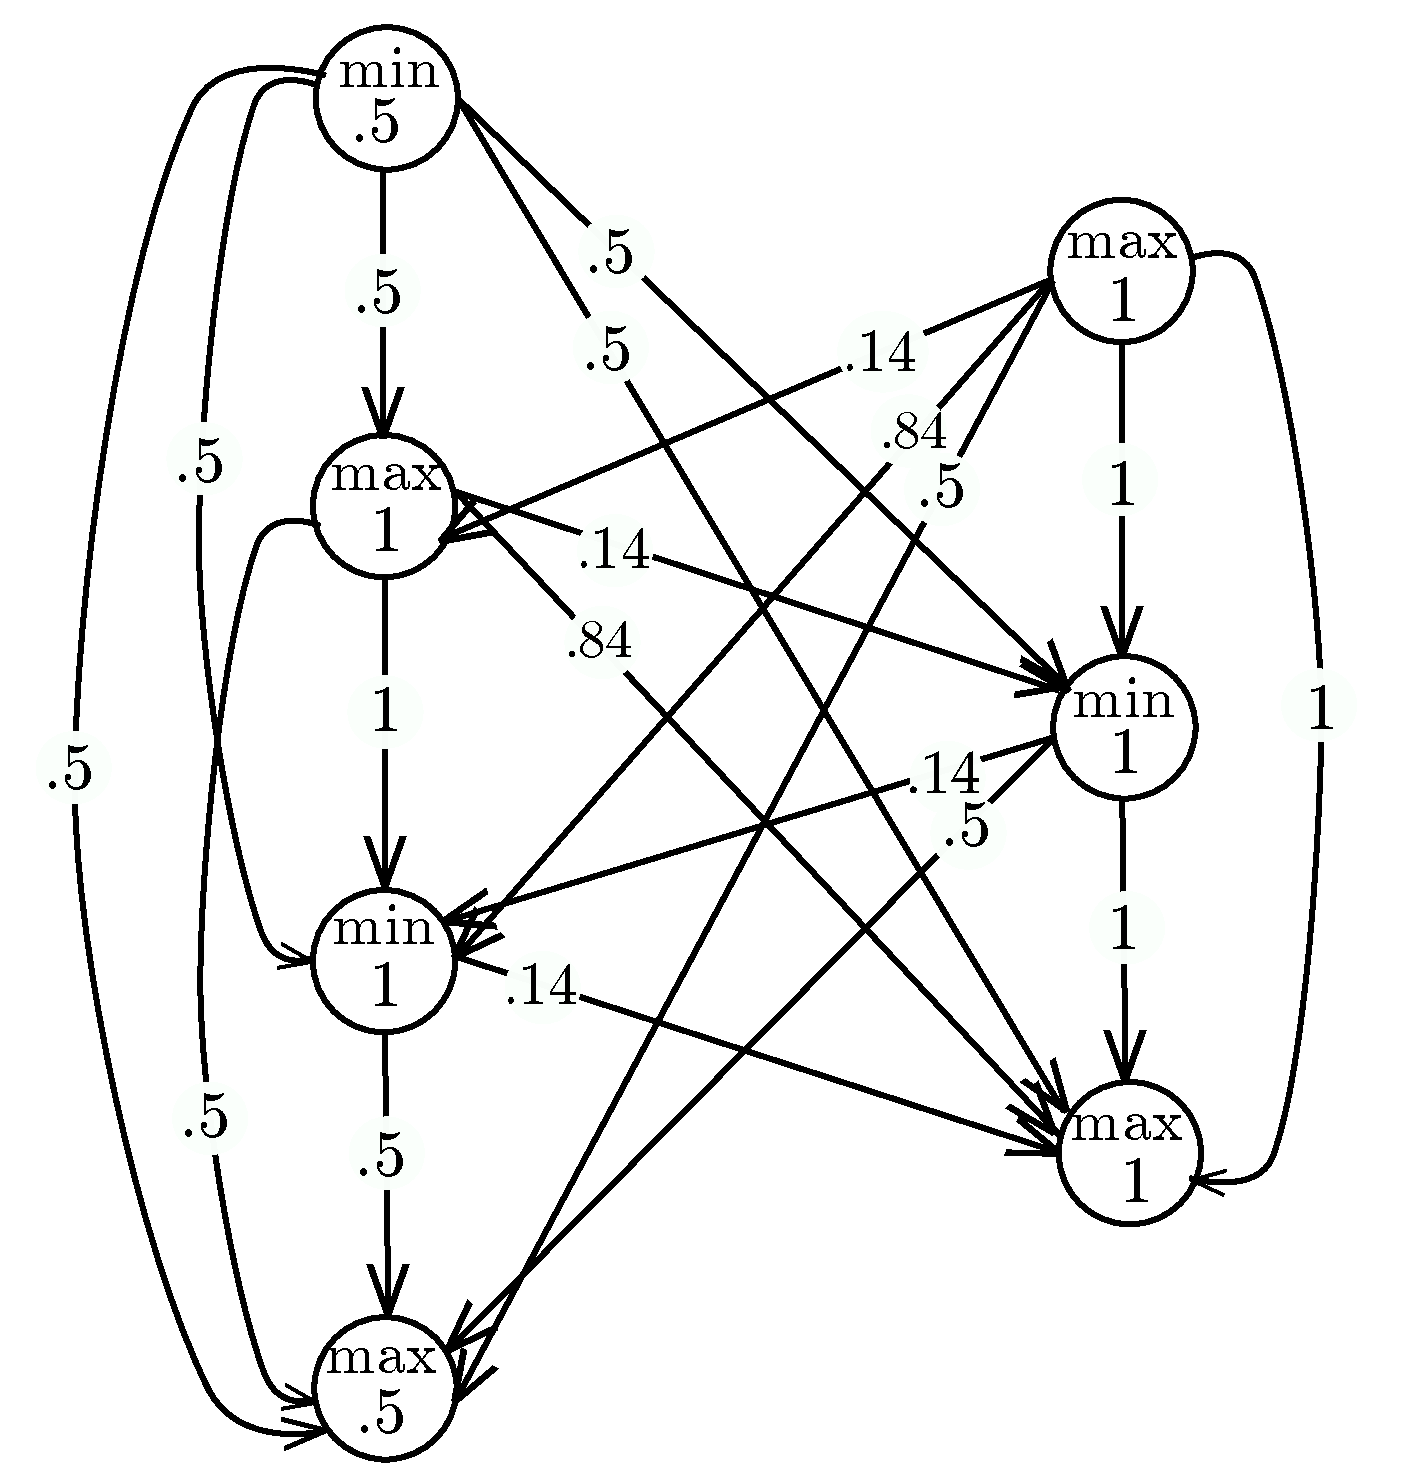
\includegraphics[width=.4\textwidth]{images/sine-unnormal.pdf}}
        \caption{Extremal Event DAG for $\sin(x):[0,2\pi]\rightarrow \R$ and $\cos(x):[0,2\pi]\rightarrow \R$.
        The nodes on the left represent the local extrema of $\sin(x)$ while the nodes on the right
        represent the local extrema of $\cos(x)$. The node weights are the node lives of the corresponding
        local extrema while the edge weights are computed using~\thmref{edge-weights}.}
        \label{fig:extremalDAGsine}
    \end{figure}
\end{example}
